\chapter{Smart Building Solution}
\label{chapter:architecture}

In this chapter there will be provided a solution to improve the efficiency and usability of a building by using automation mechanisms, enhancing the intelligence of the building. Taking in account the \ac{iot} principles, this system should be capable of real-time processing of large data streams, analyse and correlate events, and being able to react and adapt to emergency states and guarantee the minimum functionality, always. This solution is intended to integrate the SmartLightinhg project and will be addressed in this chapter.

This chapter will begin with a brief description, in section \ref{Architecture:slproject}, of SmartLighting project and its intentions of developing a smart environment of automation and control in IT2 building. Later, in order to ensure that all system necessities are addressed and taken into account, in section \ref{Architecture:Requirements} will be done a survey of necessary capabilities and  requirements to satisfy its stakeholders.

Since the main aim of this dissertation is the failure handling and adaptation of the gateways to emergency states, in section \ref{Architecture:usecases}, will be addressed three scenarios of operation needed to be taken into account.

Finally, in section \ref{Architecture:Architecture}, a presentation and evaluation of the system architecture, and its components interactions. 


\newpage


\section{SmartLighting Project}
\label{Architecture:slproject}

\subsection{Project Overview and Objectives}
\label{Architecture:Overview}

The SmartLighting project\cite{Moreira} aims to create a smart environment in IT2 building in order to automate the lighting and HVAC infrastructure. IT2 building have been running with CFL luminaries, which, are often not only, inefficient and hazardous for the environment, but also, in most cases, unable to be dimmed. 

This project intend to remove all this CFL luminaries by LED luminaries, that can resolve all the issues stated before and also are able, combining with sensors, to collect data from the environment such as luminance, temperature, humidity, motion and others. All of the collected data will be used to act in real-time to the changes in sensors readings. 

Such system needs to be backed up by an intelligent management platform in order to act based on a set of rules and input streams of sensors values. Moreover, there will be mechanisms to correlate events and determine patterns that will enable a more immediate reaction. As an example, if a user has the habit of turn on the AC everyday in the morning, the system will be able to learn and automatically do that action soon as the user arrives in the building. 

Also, the system can use external sources such as meteorological forecast to take preventively actions, such as increase the dimming levels of luminaries and the building temperature in cold rainy days.

Additionally, the users will be able to set their own rules to enhance the comfort in its office. This can be done either by using a mobile application or a web interface. Also, this user platforms can enable the use of notifications providing ways to alert the building occupants of important events. For instance, users can be informed about future meetings, the presence of another occupant in the building, and more.

Finally, an important feature for this project is the fail safe mechanisms to ensure that all the basic automation needed for the building well functioning, such as the trigger of a motion sensor lighting up the corresponding luminaries, work even if in situations of failure in core elements of the architecture or network communication problems. This can be achieved by giving gateways, the component that communicate directly with the sensors and actuators, lightweight processing mechanisms to ensure the basic functionalities described before. This will be the main focus of the presented dissertation.

\subsection{Existing Architecture}

TODO

\subsection{Stakeholders}
\label{Architecture:Stakeholders}

The success of a project depends directly in the people involved, either by developing its features or simply by consuming them in its final form. A correct identification of the stakeholders, their motivations and expectations, pay a important role in the success of any project. 

In SmartLighting project, 4 stakeholders were identified, namely:

\begin{itemize}
	\item Building occupants
	\item Building owners
	\item Building managers
	\item Developers team
\end{itemize}


The primary stakeholders in this project, are the IT2 building occupants and owners. While occupants will take direct advantage from the implemented features due to the enhance in comfort and usability of the building, owners gains will be economic as far as the building energy consumption and maintenance costs will be reduced.

As for building managers, the benefits are from easier interaction and configuration of the whole system, that allow a more precise aware of every node status, to a notification system for quicker reaction to system failures, or even to prevent such ones, and act before they happen.

Lastly, the developers team take a huge benefit in the success of the project since they are interested and devoted to create the best product possible that fulfils all the other stakeholders expectations.


\subsection{Use Cases}
\label{Architecture:SLusecases}

Based on the stakeholders survey done previously, the two main actors for this \ac{bas} solution are the building's manager and the occupants. Those actors directly use the platforms and resources provided, to enhance the comfort of the environment around them as they please, so the main focus for user driven cases will be in those two. 

Although there are many use cases for both the building's manager and the occupants, in this section will be only addressed those that were already implemented in this project, giving a greater understanding of the overall project's functionalities. Later in section \ref{Architecture:usecases}, there will be presented the use cases and scenarios introduced by this dissertation work.

\begin{Paragraph}{Building occupant}
	
The building occupants will be the principal users that will interact with the system. This interaction can be achieved by using either a mobile application or a web interface. The use cases addressed bellow combine the most common and frequent operations:


\begin{figure}[H]
	\centering
	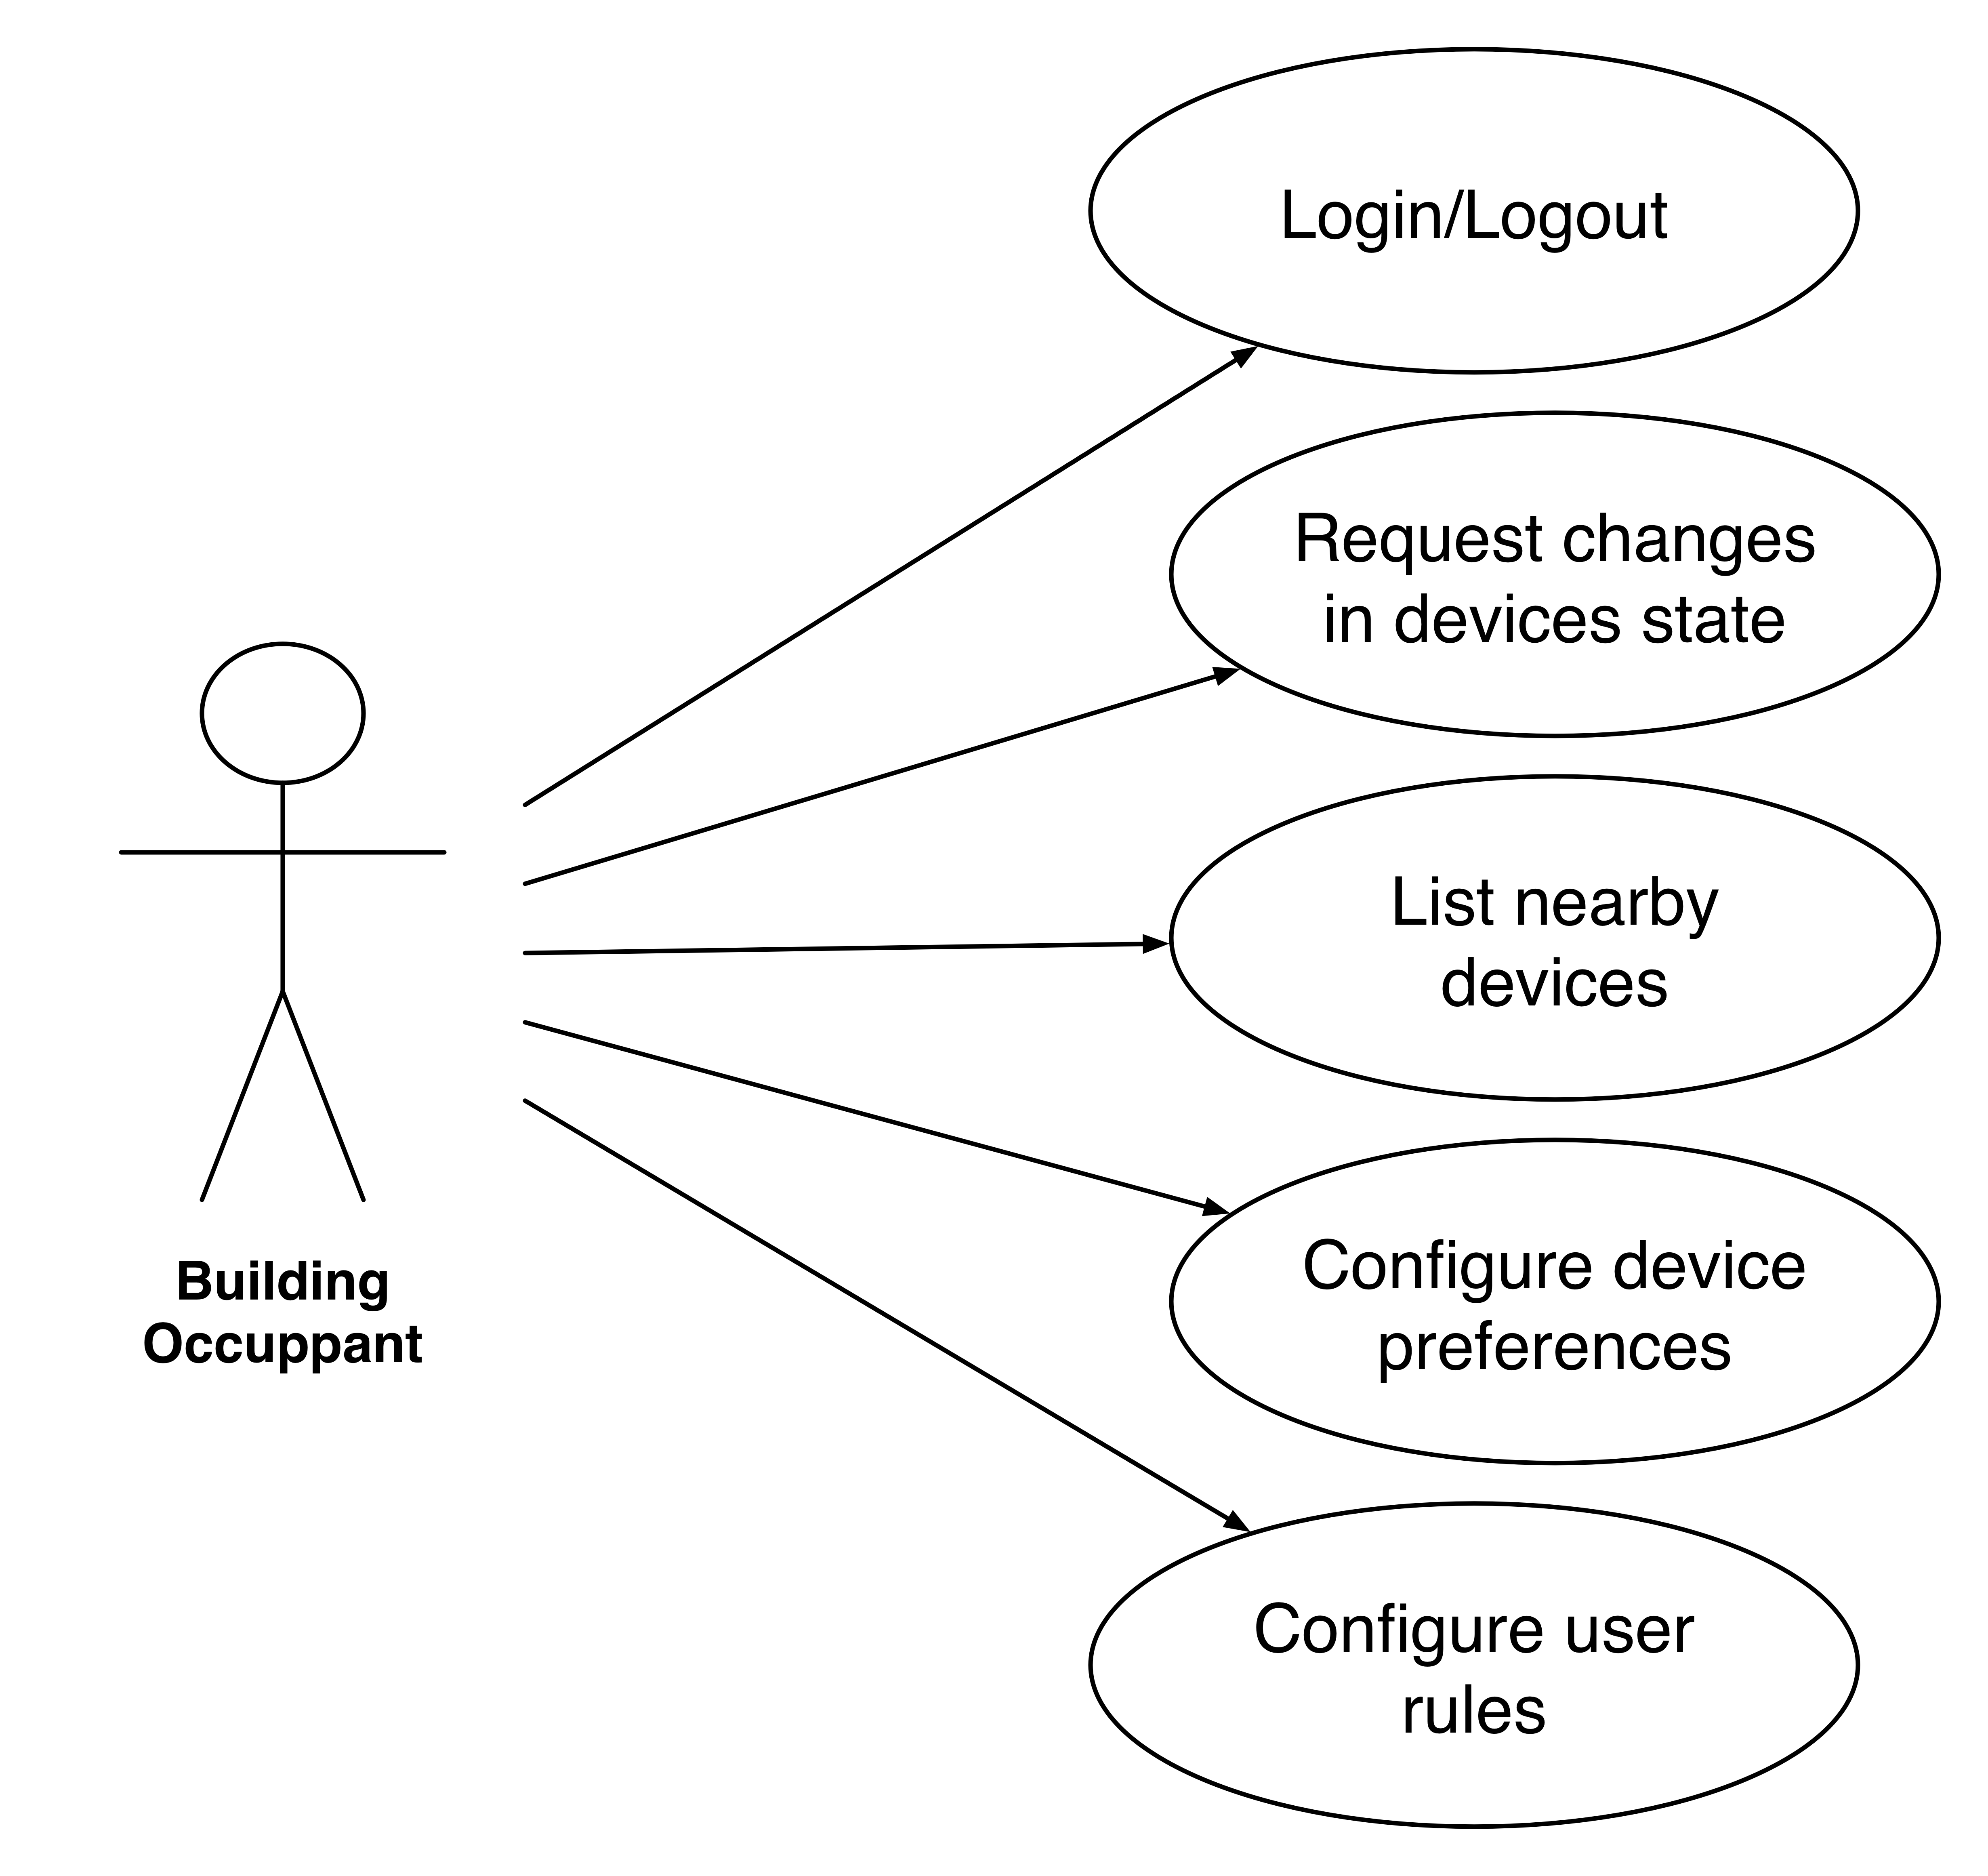
\includegraphics[width=0.5\textwidth]{figures/usecase1.png}
	\caption{Use case diagram of building occupants interaction with the system.}
	\label{fig:user}
\end{figure}

\begin{itemize}

	\item{\textbf{Login/Logout:}	This use cases are intended to enable the access to user oriented features. The building occupants can login in the platform, either using the mobile application or the web interface, to access his preferences and personal environment control features.}
	\item{\textbf{Request changes in devices state:}	The building occupant can request a change in the state of a device, that can be accepted or denied by the system depending on the access rights of the user. For instance, an occupant can request a change in near by devices like  air conditioners, lights, and others.}
	\item{\textbf{List nearby devices:}	This use case allows users to request the list of nearby devices, based on its location, allowing to access or request changes to devices in the same room as the occupant, giving that these are the most likely to be needed access.}
	\item{\textbf{Configure device preferences:}	The user can create or edit device pre-sets, allowing that the selected values are applied automatically to the device in future uses. For instance, the air conditioner in a user office can be pre-set to 21ºC so that when this device is turned on, that value is automatically set. This changes would also depend with the user access rights.}
	\item{\textbf{Configure user rules:}	This use case allow the building occupants to create rules that preform a set of actions automatically, giving the right conditions. For instance the user could create a rule to automatically turn the air conditioner on if the temperature in his office exceed a giving value.} 

\end{itemize}
\end{Paragraph}


\begin{Paragraph}{Building manager}
	
	
	\begin{figure}[H]
		\centering
		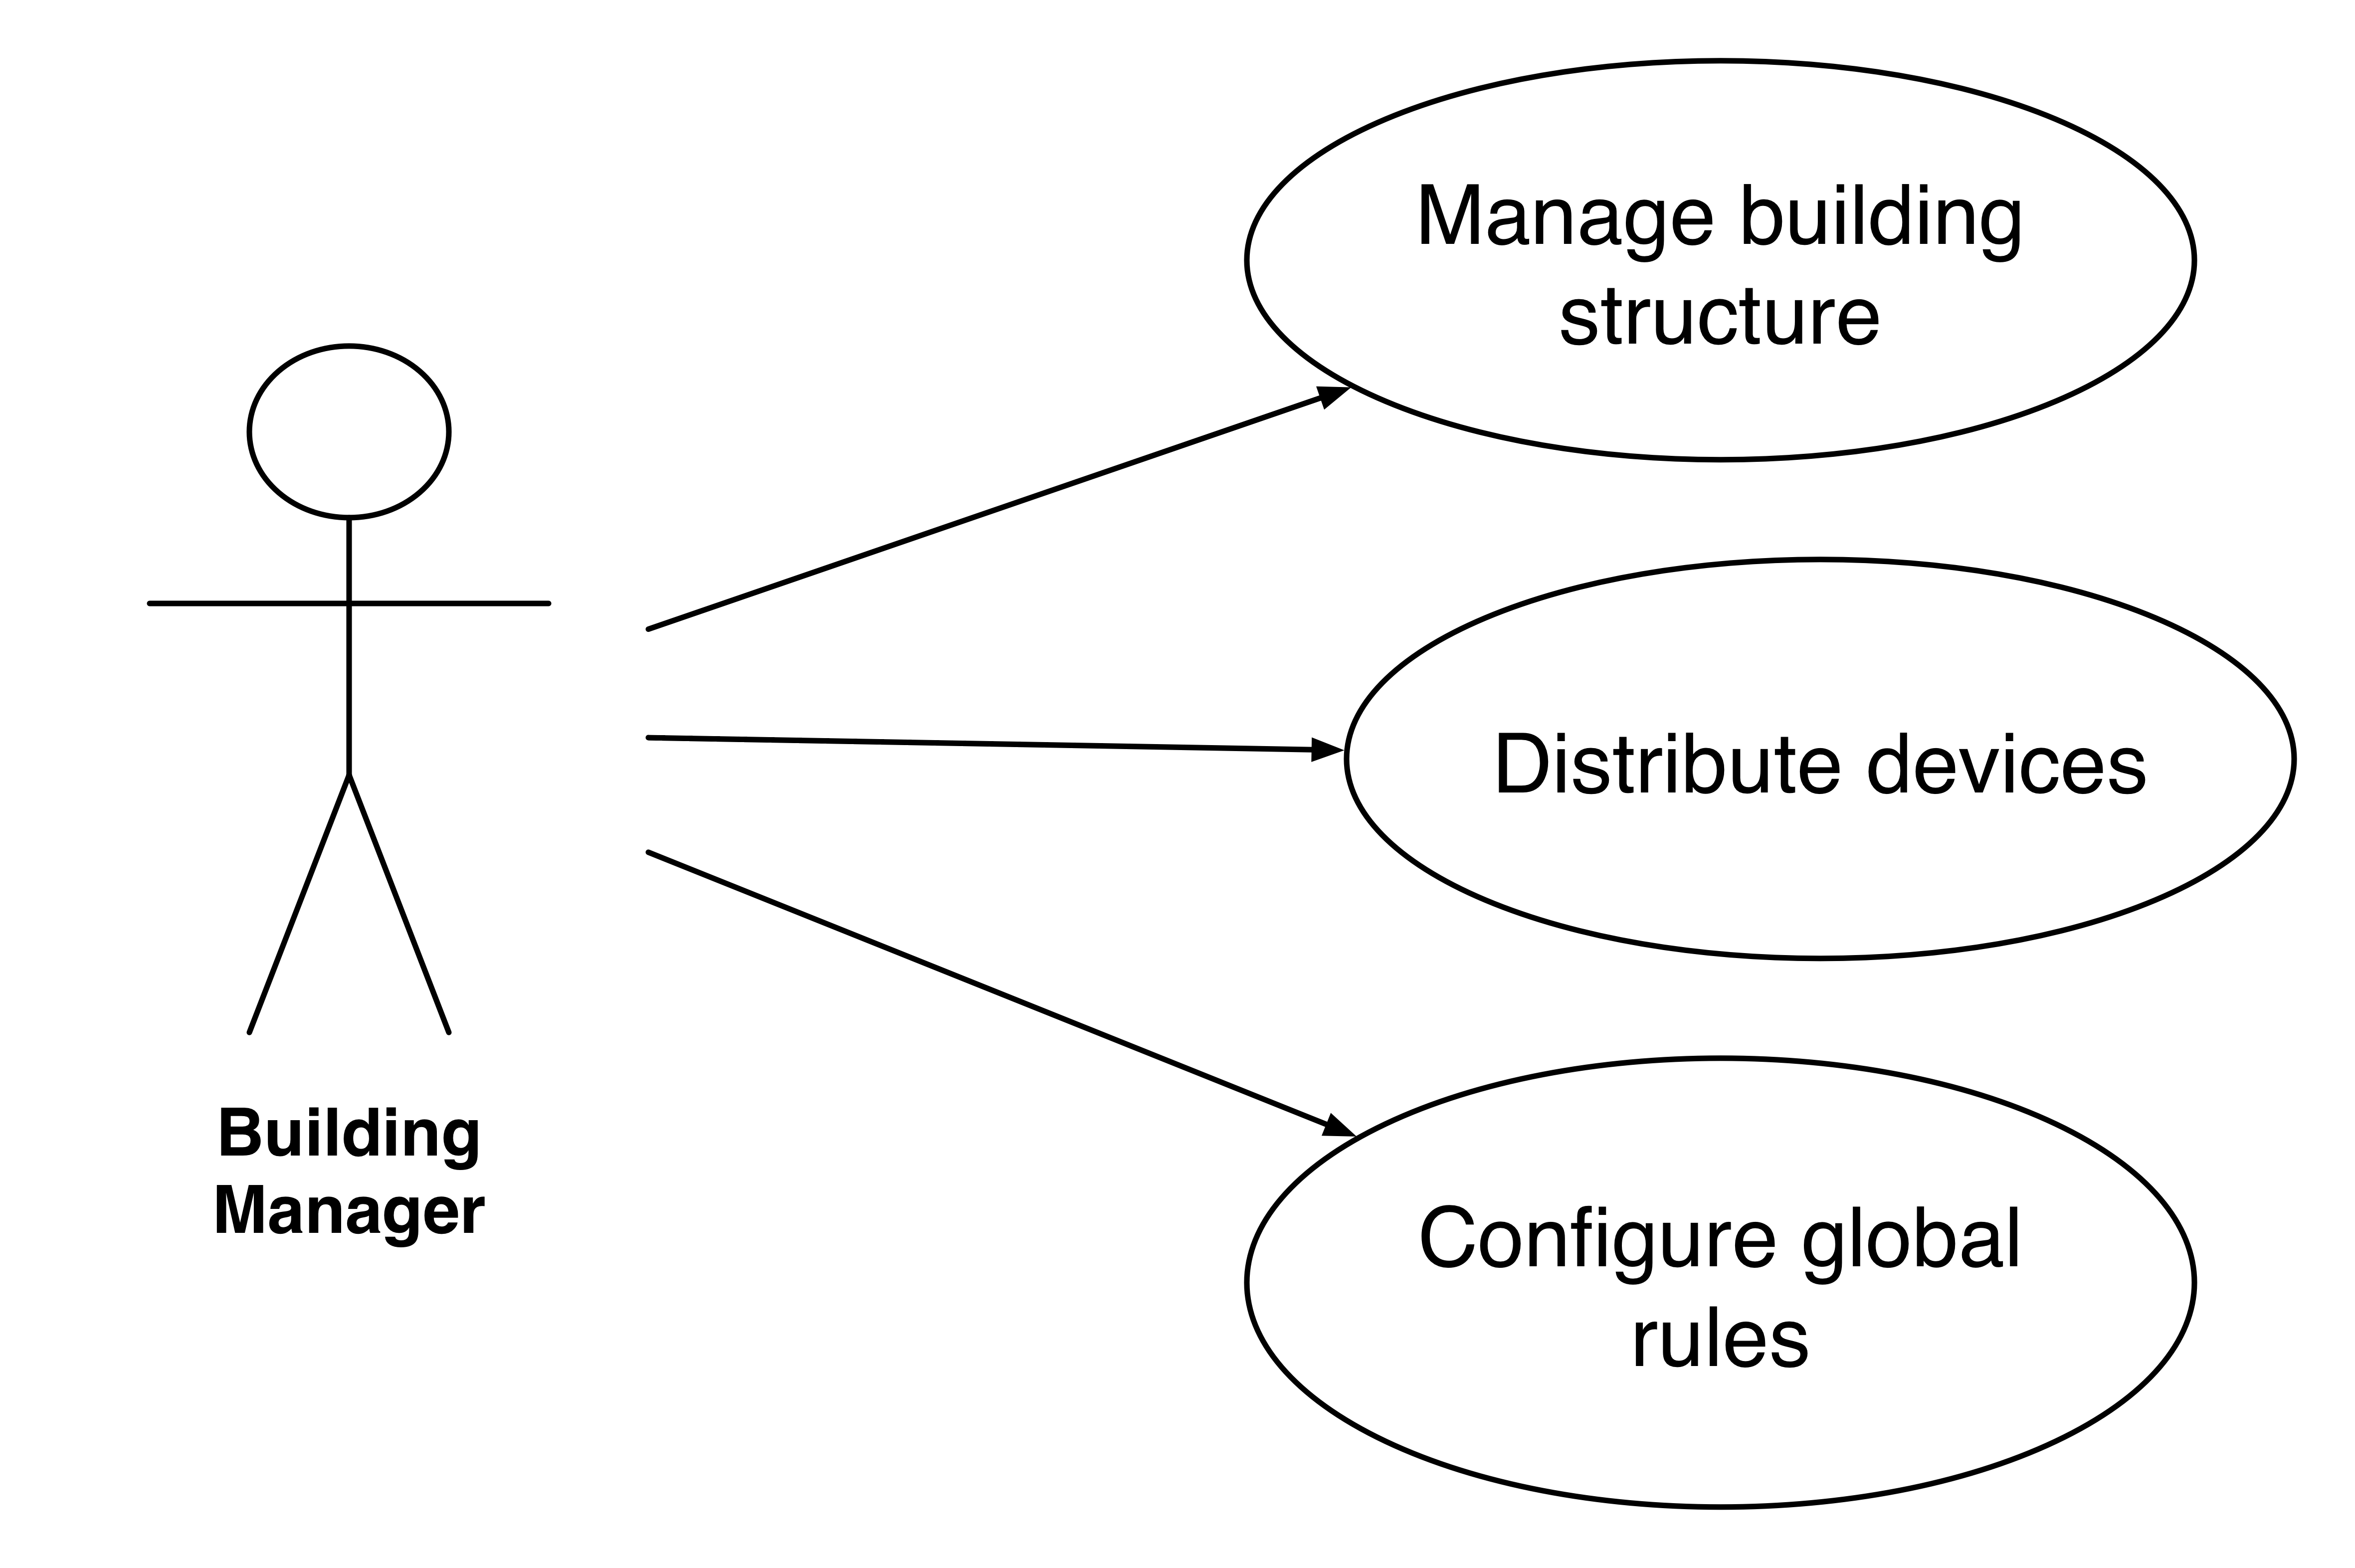
\includegraphics[width=0.5\textwidth]{figures/usecase2.png}
		\caption{Use case diagram of building manager interaction with the system.}
		\label{fig:manager}
	\end{figure}
\begin{itemize}
	\item{\textbf{Manage building structure:}	The manager can create the representation of the building in the structure management platform. This allow the creation of a virtual portrayal of the floors, rooms and areas of the building.}
	\item{\textbf{Distribute devices:}	This use case permit that connected devices can be distributed through the areas and rooms of the building virtual representation.}
	\item{\textbf{Configure global rules:}	The building manager has the ability to add, delete, enable or disable rules for the whole building. These core rules' main purpose are the building's efficiency increase, for instance instead of leaving the corridors lights always on, a rule can be created to turn them off when there's no one walking by. There is also a mechanism to test the rule before the deployment.}
\end{itemize}
\end{Paragraph}


\section{System Architecture}
\label{Architecture:Architecture}


Taking into account the objectives for this dissertation, and the existing architecture for the SmartLighting project, the proposed architecture has in mind, not only \ac{iot} and complex event processing principles, but also the referred features for this dissertation such as failure handling and rules distribution through gateways.

In this section will be presented the global system architecture for this project, represented in Figure \ref{fig:arch} as well as a description of all the components that compose the solution.

Note that components like the \ac{cep} engine, and the \ac{bm} are already implemented due to a past dissertation for the SmartLighting project \cite{helder}.

\begin{figure}[H]
	\centering
	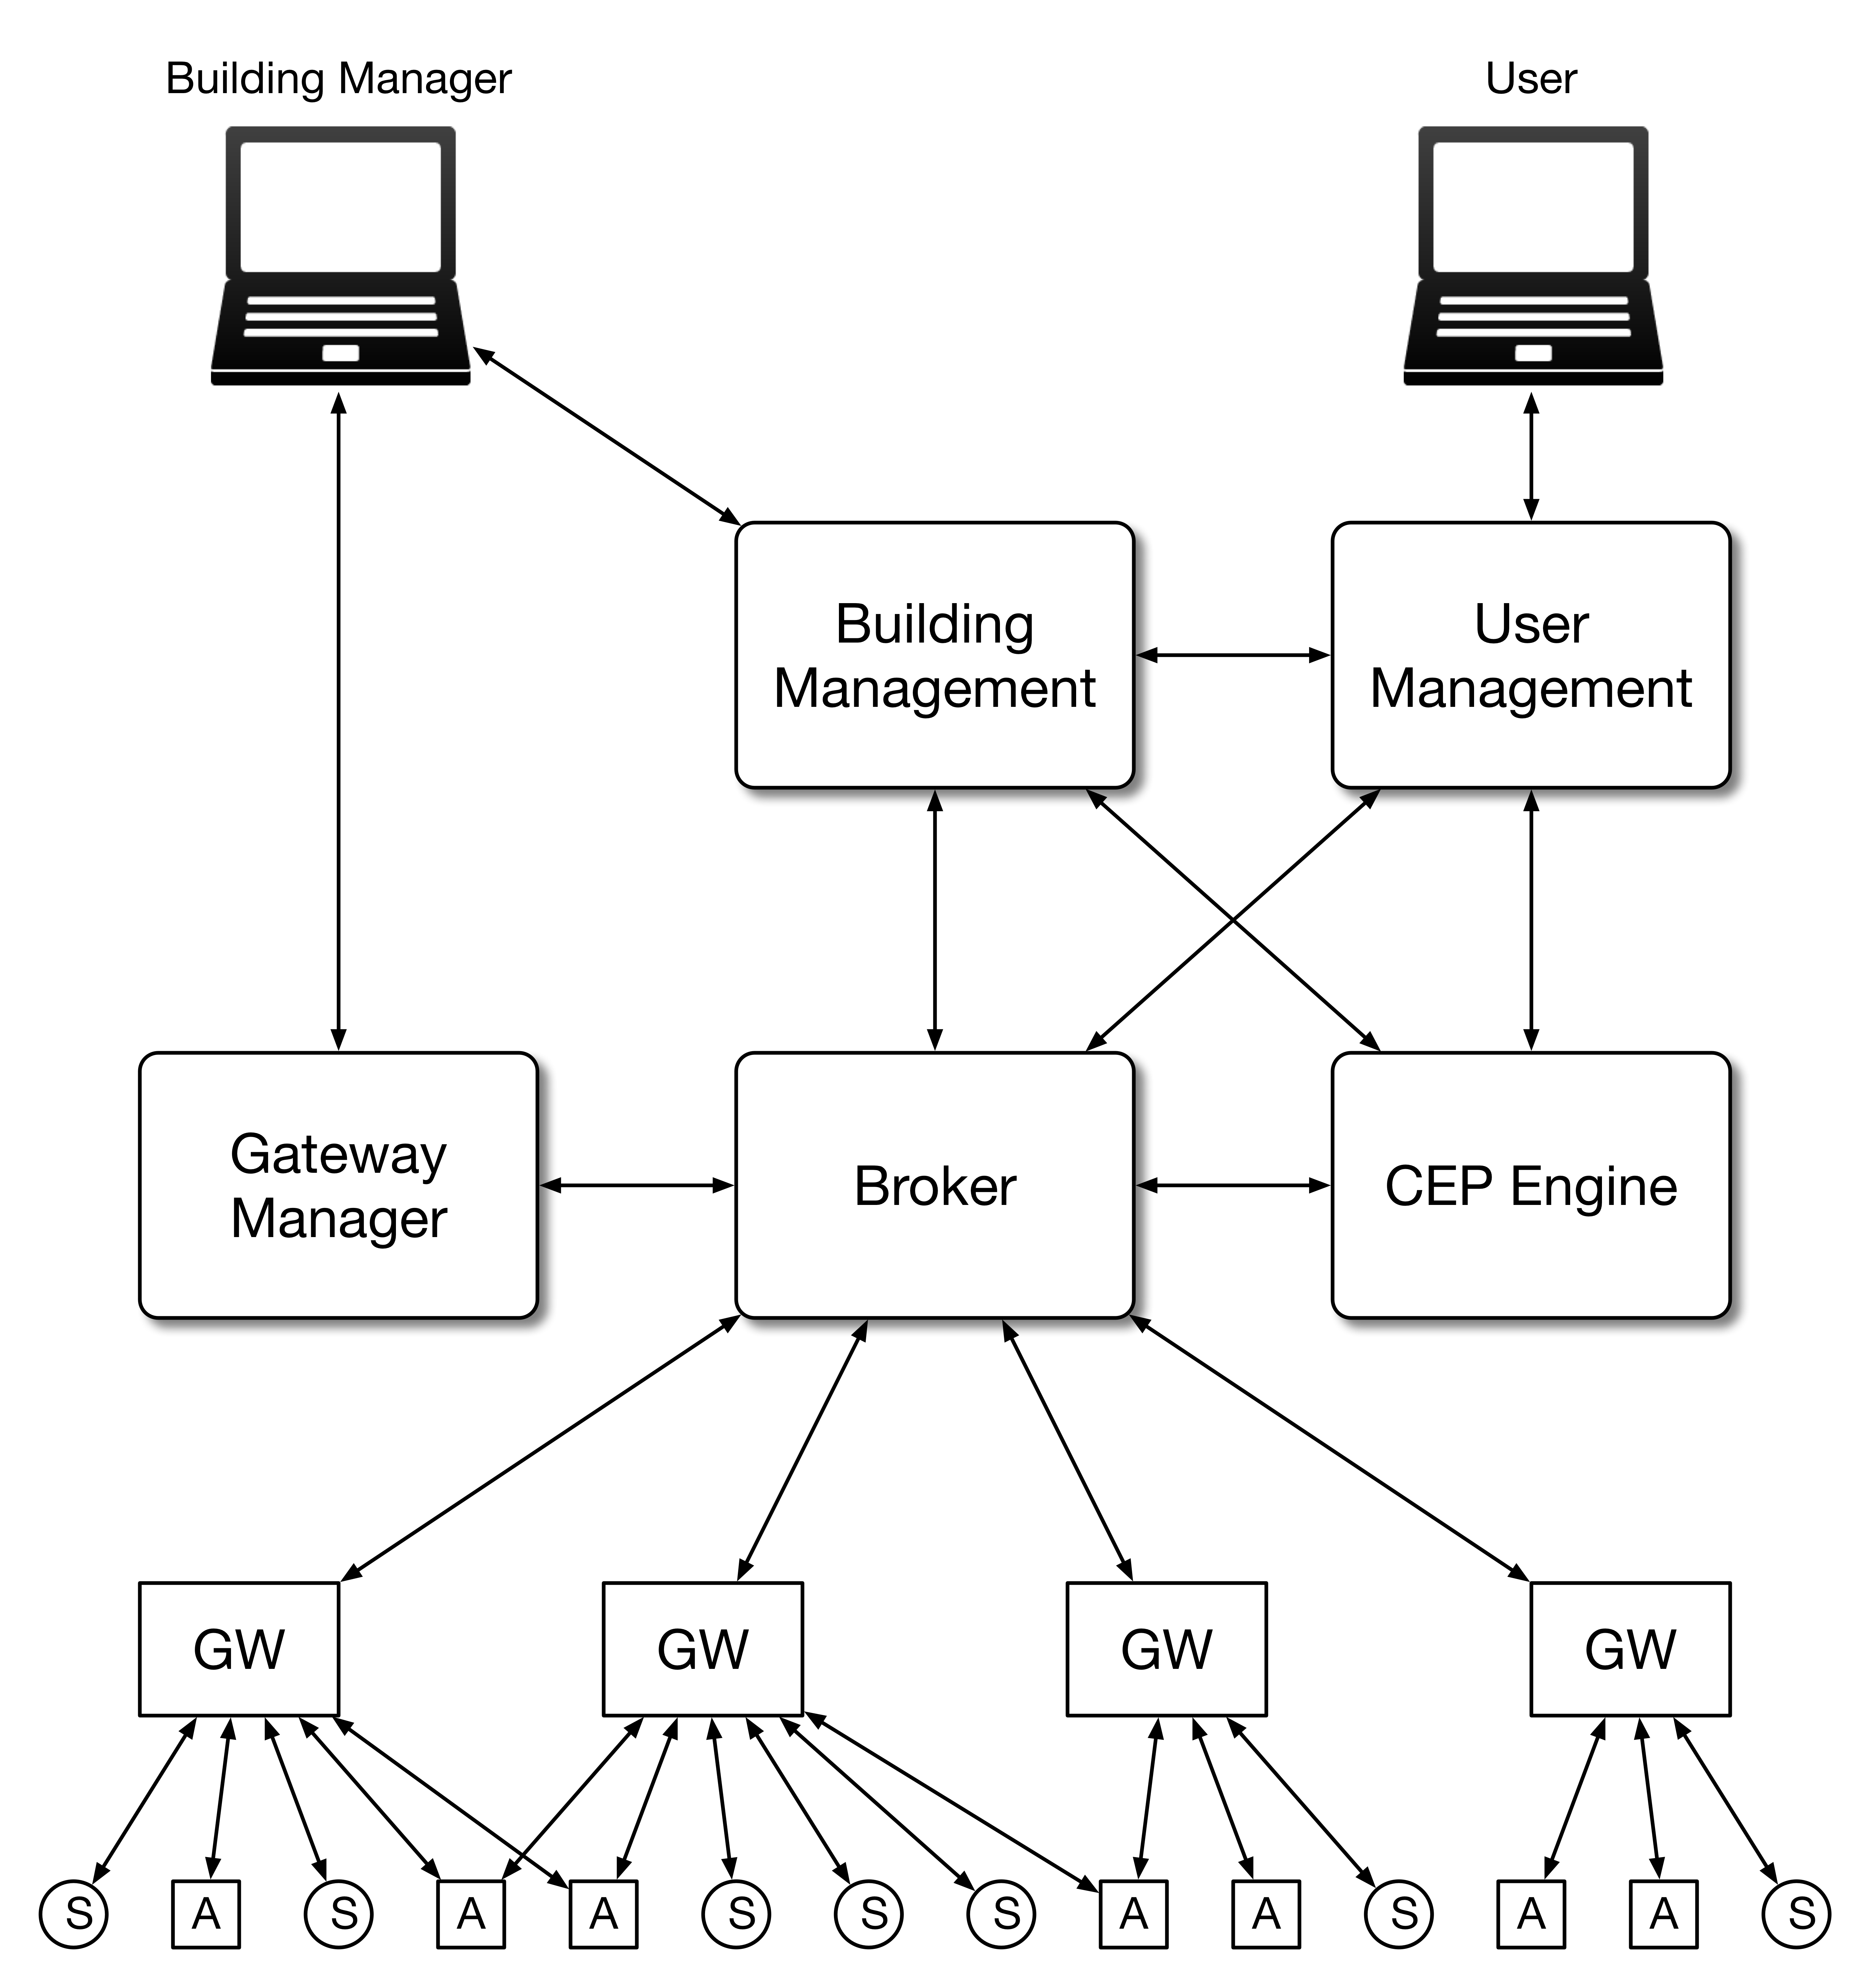
\includegraphics[width=0.9\textwidth]{figures/architecture.png}
	\caption{Smart Building: Architecture diagram}
	\label{fig:arch}
\end{figure}



\subsection{Components Overview}

\begin{Paragraph}{User Management}
	
	The user management platform is responsible for giving to common users of the building, the ability to interact with the platform through a web page. Users can manage their own building rules and control field devices directly. This can be done by publishing on the broker the wanted changes or by communication directly with the CEP Engine or the building management platform.
	
\end{Paragraph}

\begin{Paragraph}{Building Management}
	
	The building manager component is a user friendly platform that aims to facilitate the rule management and the configuration of the building's schema. The building manager can create, edit  or delete rules in a simple intuitive way and this component later translates them in a complex language that the CEP Engine can understand. Also, through a virtual representation of the building, the \ac{bm} can distribute devices across all its areas. After the correct configuration of the desired devices, this component is responsible for providing the information about each device and how should the CEP engine, and the other blocks of the architecture, address to this device in order to, for instance, send an order to change state or report new sensor data to the CEP Engine.
	
\end{Paragraph}

\begin{Paragraph}{CEP Engine}
	
	The CEP Engine is one of the most important components for a successful building automation solution. This engine must be a real-time and high performance component, that should be able to process hundreds of sensor triggered events per second based on complex rules created by the users. The actions preformed by this engine can be either directly to an actuator or to a component in the platform. For instance, sending an alert to the building manager when there are irregular sensor readings.
	
	
\end{Paragraph}

\begin{Paragraph}{Broker}
	
	The broker component, which refers to a message broker, it is responsible for receive and route information across the connected components. Every component connects to receive and send information, to and from other components.
	
\end{Paragraph}

\begin{Paragraph}{Gateway Manager}
	
	The gateway manager is the component responsible for rules distribution to gateways and fail handling. The first one, since gateways will be equipped with the ability to process events, based on simple rules in the case of CEP failure, there is the need for a regulator to distribute and be always aware where this rules are being deployed, and, in case of a gateway failure, distribute the devices and rules from that gateway, to other ones capable of supporting them. Also, the gateway manager should guarantee a balanced number of rules and devices across all gateways. For instance, if two gateways are in the reach of the same device, the gateways manager should allocate that device to the gateway with fewer devices.
	
	
\end{Paragraph}

\begin{Paragraph}{Gateways}
	
	Gateways are responsible for discovering devices and communicate to them. This nodes have to convert sensor's events into understandable messages to the automation engine, and vice versa. Also, gateways should be equipped with a lightweight automation engine so that, in case of a failure in the CEP Engine or in the broker, the gateways can continue to process events, and thus, a minimum downtime in the system's functioning.
	
\end{Paragraph}

\begin{Paragraph}{Sensors and actuators}
	
	The field layer represents the set of devices, both sensors and actuators, used to gather information and interact with the environment. The information gathering and detection of changes is done by sensors, that send this information to the respective gateways in the Network layer. After the processing of this data, either in the Aggregation and Automation layer or even by the gateways in the Network layer, the orders for changes are sent to the actuators.
	
\end{Paragraph}

\section{Requirements}
\label{Architecture:Requirements}
As stated before, the proposed solution for this dissertation is part of the SmartLighting project, thus, designed to be integrated in a real-world scenario. Accordingly, the requirements, in this section, must converge and be in conformity with the project's objectives stated in section \ref{Architecture:slproject}. 

\begin{Paragraph}{Fast Responsiveness}

The system's performance and fast responsiveness are huge requirements for a successful \ac{bas} solution. The system must react to events with such responsiveness that the occupants experience and comfort is not affected. For instance, when a user enters a room, it is expects that the lights turn on in a question of milliseconds causing an instantaneousness feeling to the user. In other cases, a slower responsiveness is not critical for the occupant. As an example, in the heating system, when the temperature goes bellow a certain threshold, if the air conditioners take a few seconds to turn on, it won't be noticeable for the users.

In addiction, the system's management platform responsiveness is another performance requirement as it shouldn't feel slow to the user.

\end{Paragraph}

\begin{Paragraph}{Flexibility}

One important requirement for this project is flexibility. Firstly, in order to have a system that can be easily upgradable, components must be independent of hardware. For instance, the gateway software must be developed in such way that can work in a large number of micro-controllers and  low power \ac{soc} computer. Also, the communication protocols between system components should be able to be changed allowing to meet different requirements of different scenarios. 


Finally, the system should facilitate the integration of different type of sensors or actuators, without the need verbose and difficult configurations.

\end{Paragraph}

\begin{Paragraph}{Scalability}

The system should assure that with the addition of devices, the overall performance does not decline. Also, it should facilitate the horizontal scalability of system nodes, making it transparent and easy to integrate new servers to maintain or improve the system's performance.

\end{Paragraph}

\begin{Paragraph}{Failure Handling and Basic Functionalities}
	
Failure handling and the assurance of basic functionalities were the main goals for this dissertation, making very important, the requirements regarding this topic.

The whole system is designed to fulfil a set of expectations and to work perfectly at any given time, however, there could be some cases where due to a critical system failure, either a downtime in the CEP engine, communication errors or a congested network, the whole system could start malfunctioning. In more severe cases this could mean, for instance, an entire blackout in a building, or a fire sensor not triggering the alarm leading to serious injuries to the occupants.

With all this facts in consideration, a significant requirement for a \ac{bas} solution is the ability to be always aware of the entire system state and to react immediately to abnormal system occurrences. This means, for instance, that in case of communication failure between the sensors and the \ac{cep} engine, the basic functionalities like lights turning on or off, alarms, doors and other key functionalities still work autonomously.
\end{Paragraph}

\begin{Paragraph}{Data Correlation}

In order to a more accurate and elaborate reaction to sensing events, the event processing unit should be able to correlate events and infer decisions based on previous learning. For instance, if a user always turn on the air conditioner, when the temperature is bellow a certain threshold, the system should be able to learn from this behaviour and promptly react without human intervention.

\end{Paragraph}

\begin{Paragraph}{User Control and User-friendly Interfaces}
	
The system should allow users, based on their roles and permissions, to manually alter the state of a device. This means that interfaces, web or mobile, should be available to the users to control the surroundings. This interfaces should be done, taking in account that not all users have the expertise to interact with verbose configuration parameters, thus, the interfaces should be as intuitive and perceptible as possible.
	
\end{Paragraph}




\section{Failure Use Cases}
\label{Architecture:usecases}

In order to achieve an environment where the minimum functionality of the system is always assured, for example, the lights turning on when someone walks in a corridor, there can be no system component that, in case of failure, could put in risk those functionalities. With this in mind, and looking to the existing architecture, simplified in Figure \ref{fig:sc1} only with components that directly and actively affect the event processing capability, three operation scenarios can be identified. 


\begin{Paragraph}{Scenario 1 - All components are operational}
	
	\begin{figure}[H]
		\centering
		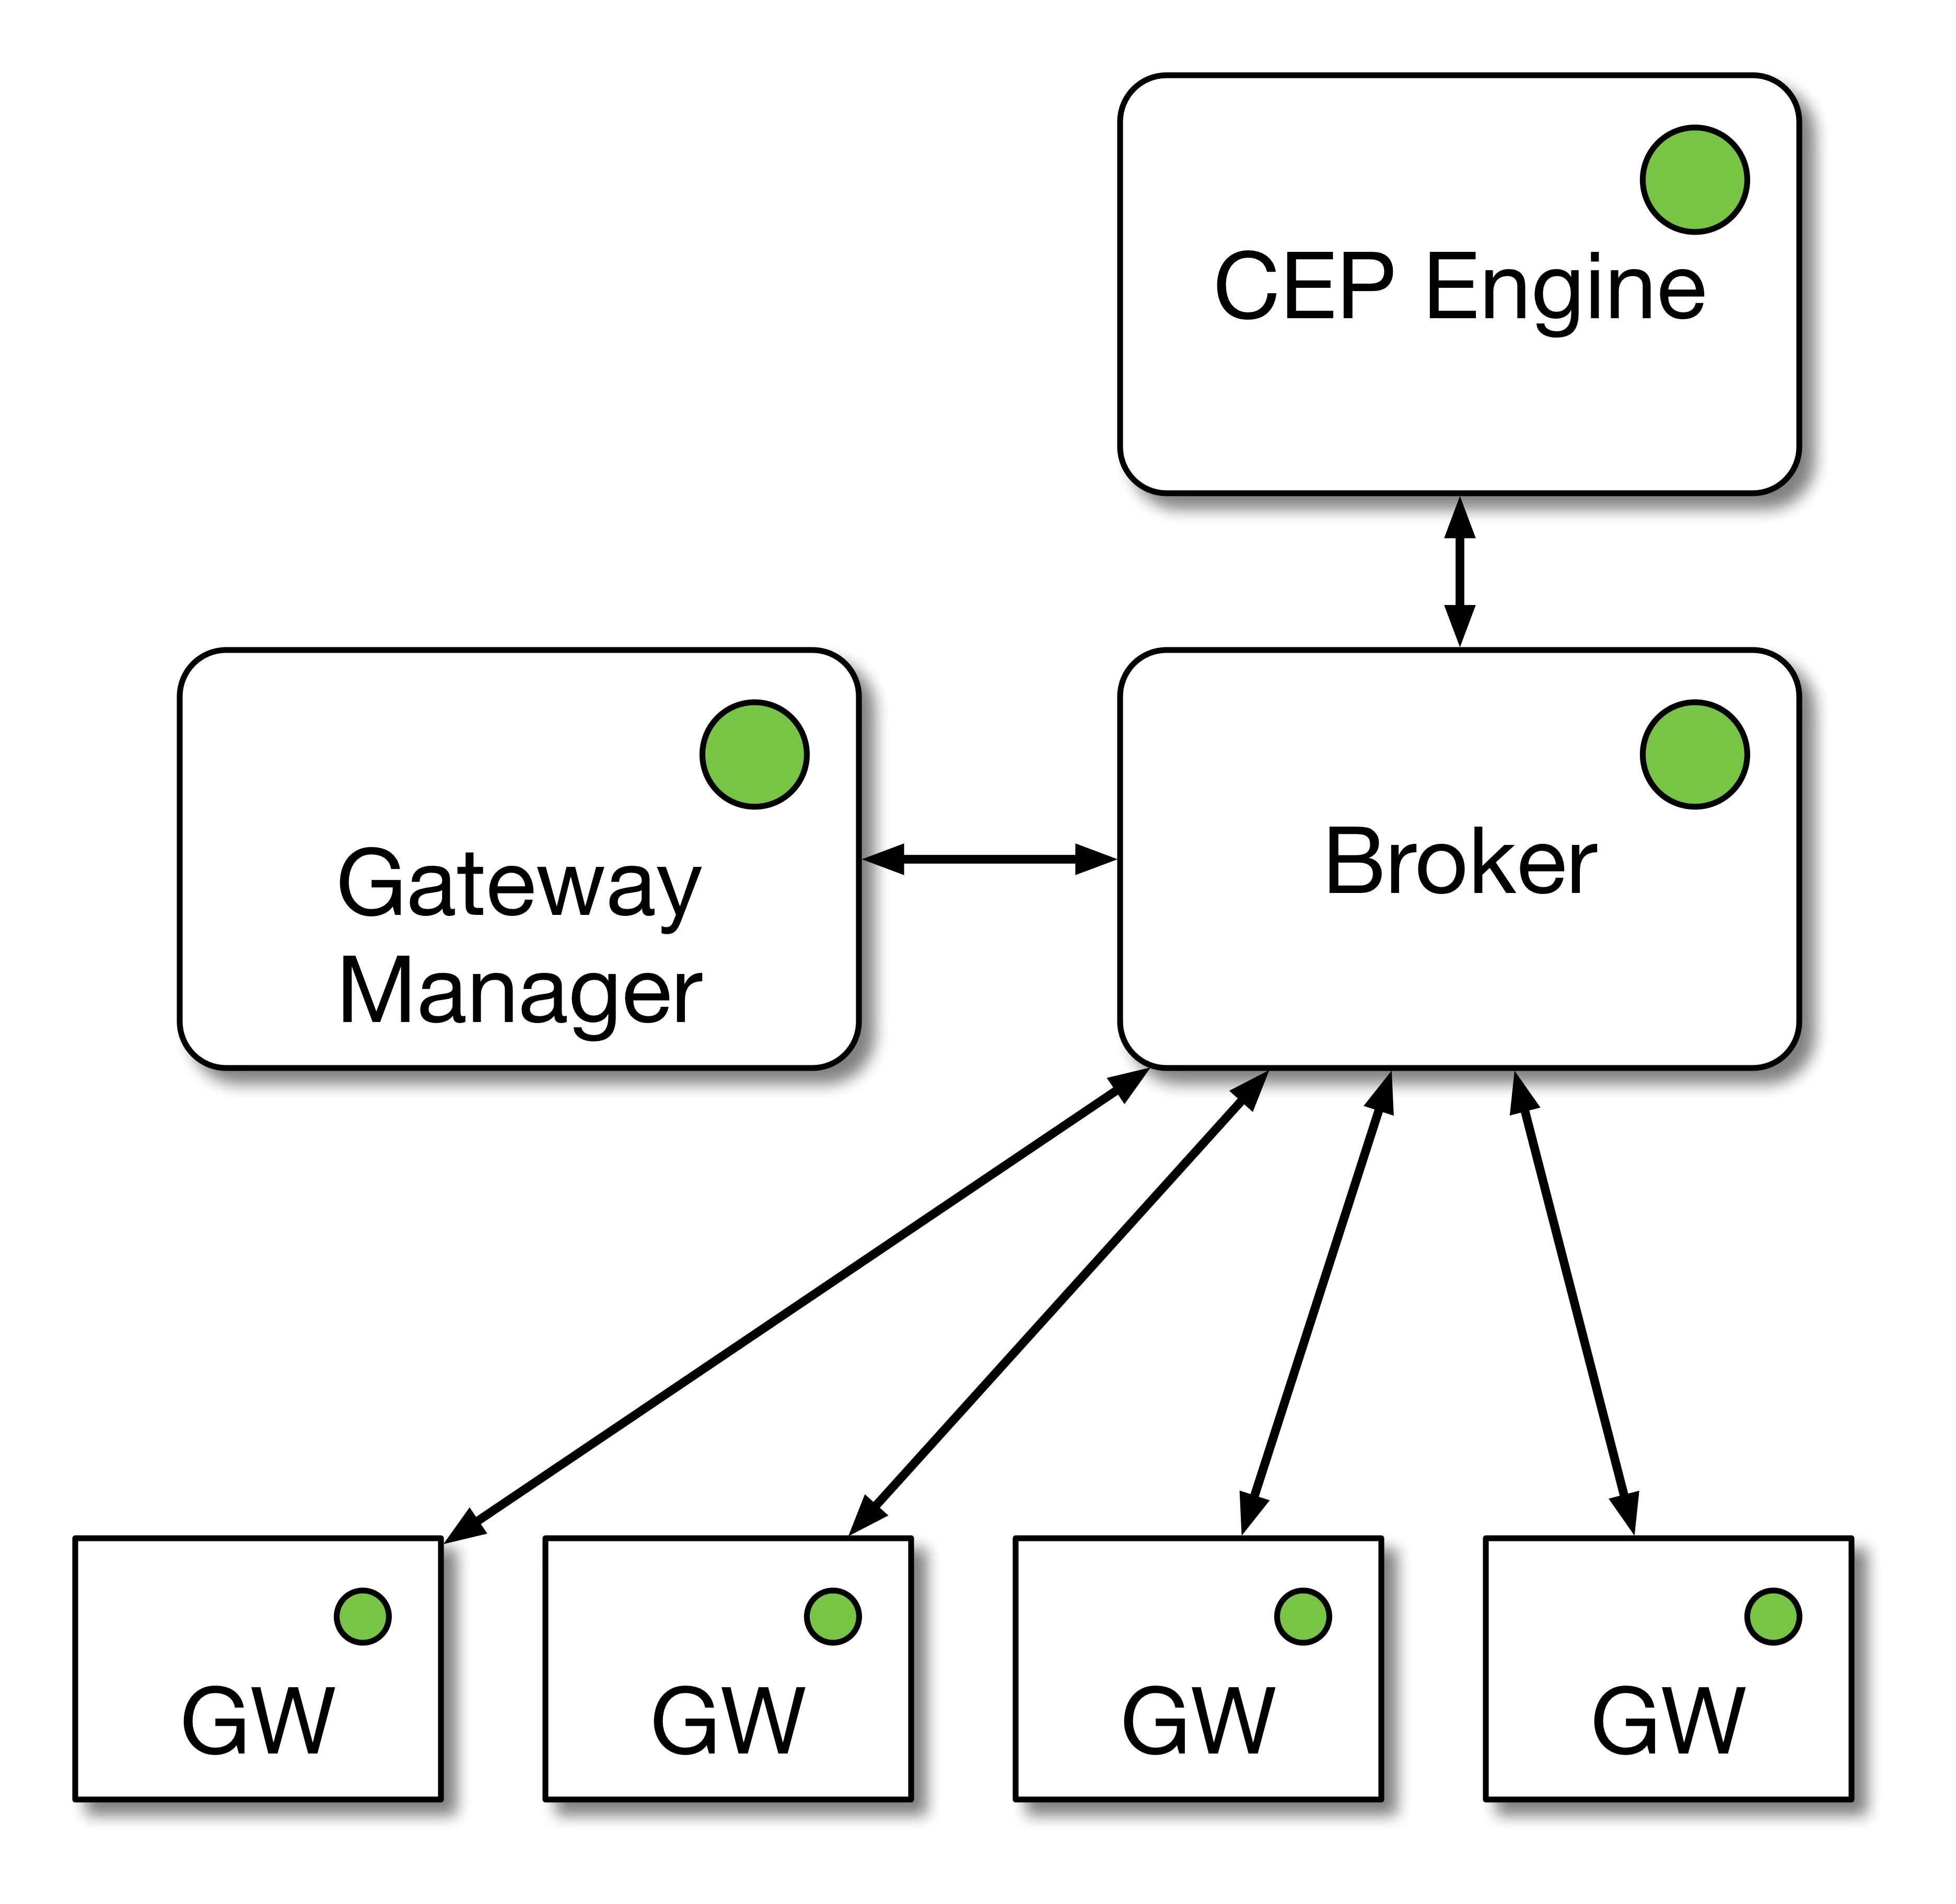
\includegraphics[width=0.4\textwidth]{figures/fs1.png}
		\caption{Simplified SmartLighting architecture.}
		\label{fig:sc1}
	\end{figure}
	
	This first scenario corresponds to the normal operation of the system, as shown in Figure \ref{fig:sc1}, where every component is working properly. In this case, the CEP module should receive events, generated by devices and sent to the message broker by gateways, process them and send the result to the message broker, and later to the corresponding gateway. 
	
	
	
\end{Paragraph}

\begin{Paragraph}{Scenario 2 - \ac{cep} Engine failure}
	
		\begin{figure}[H]
		\centering
		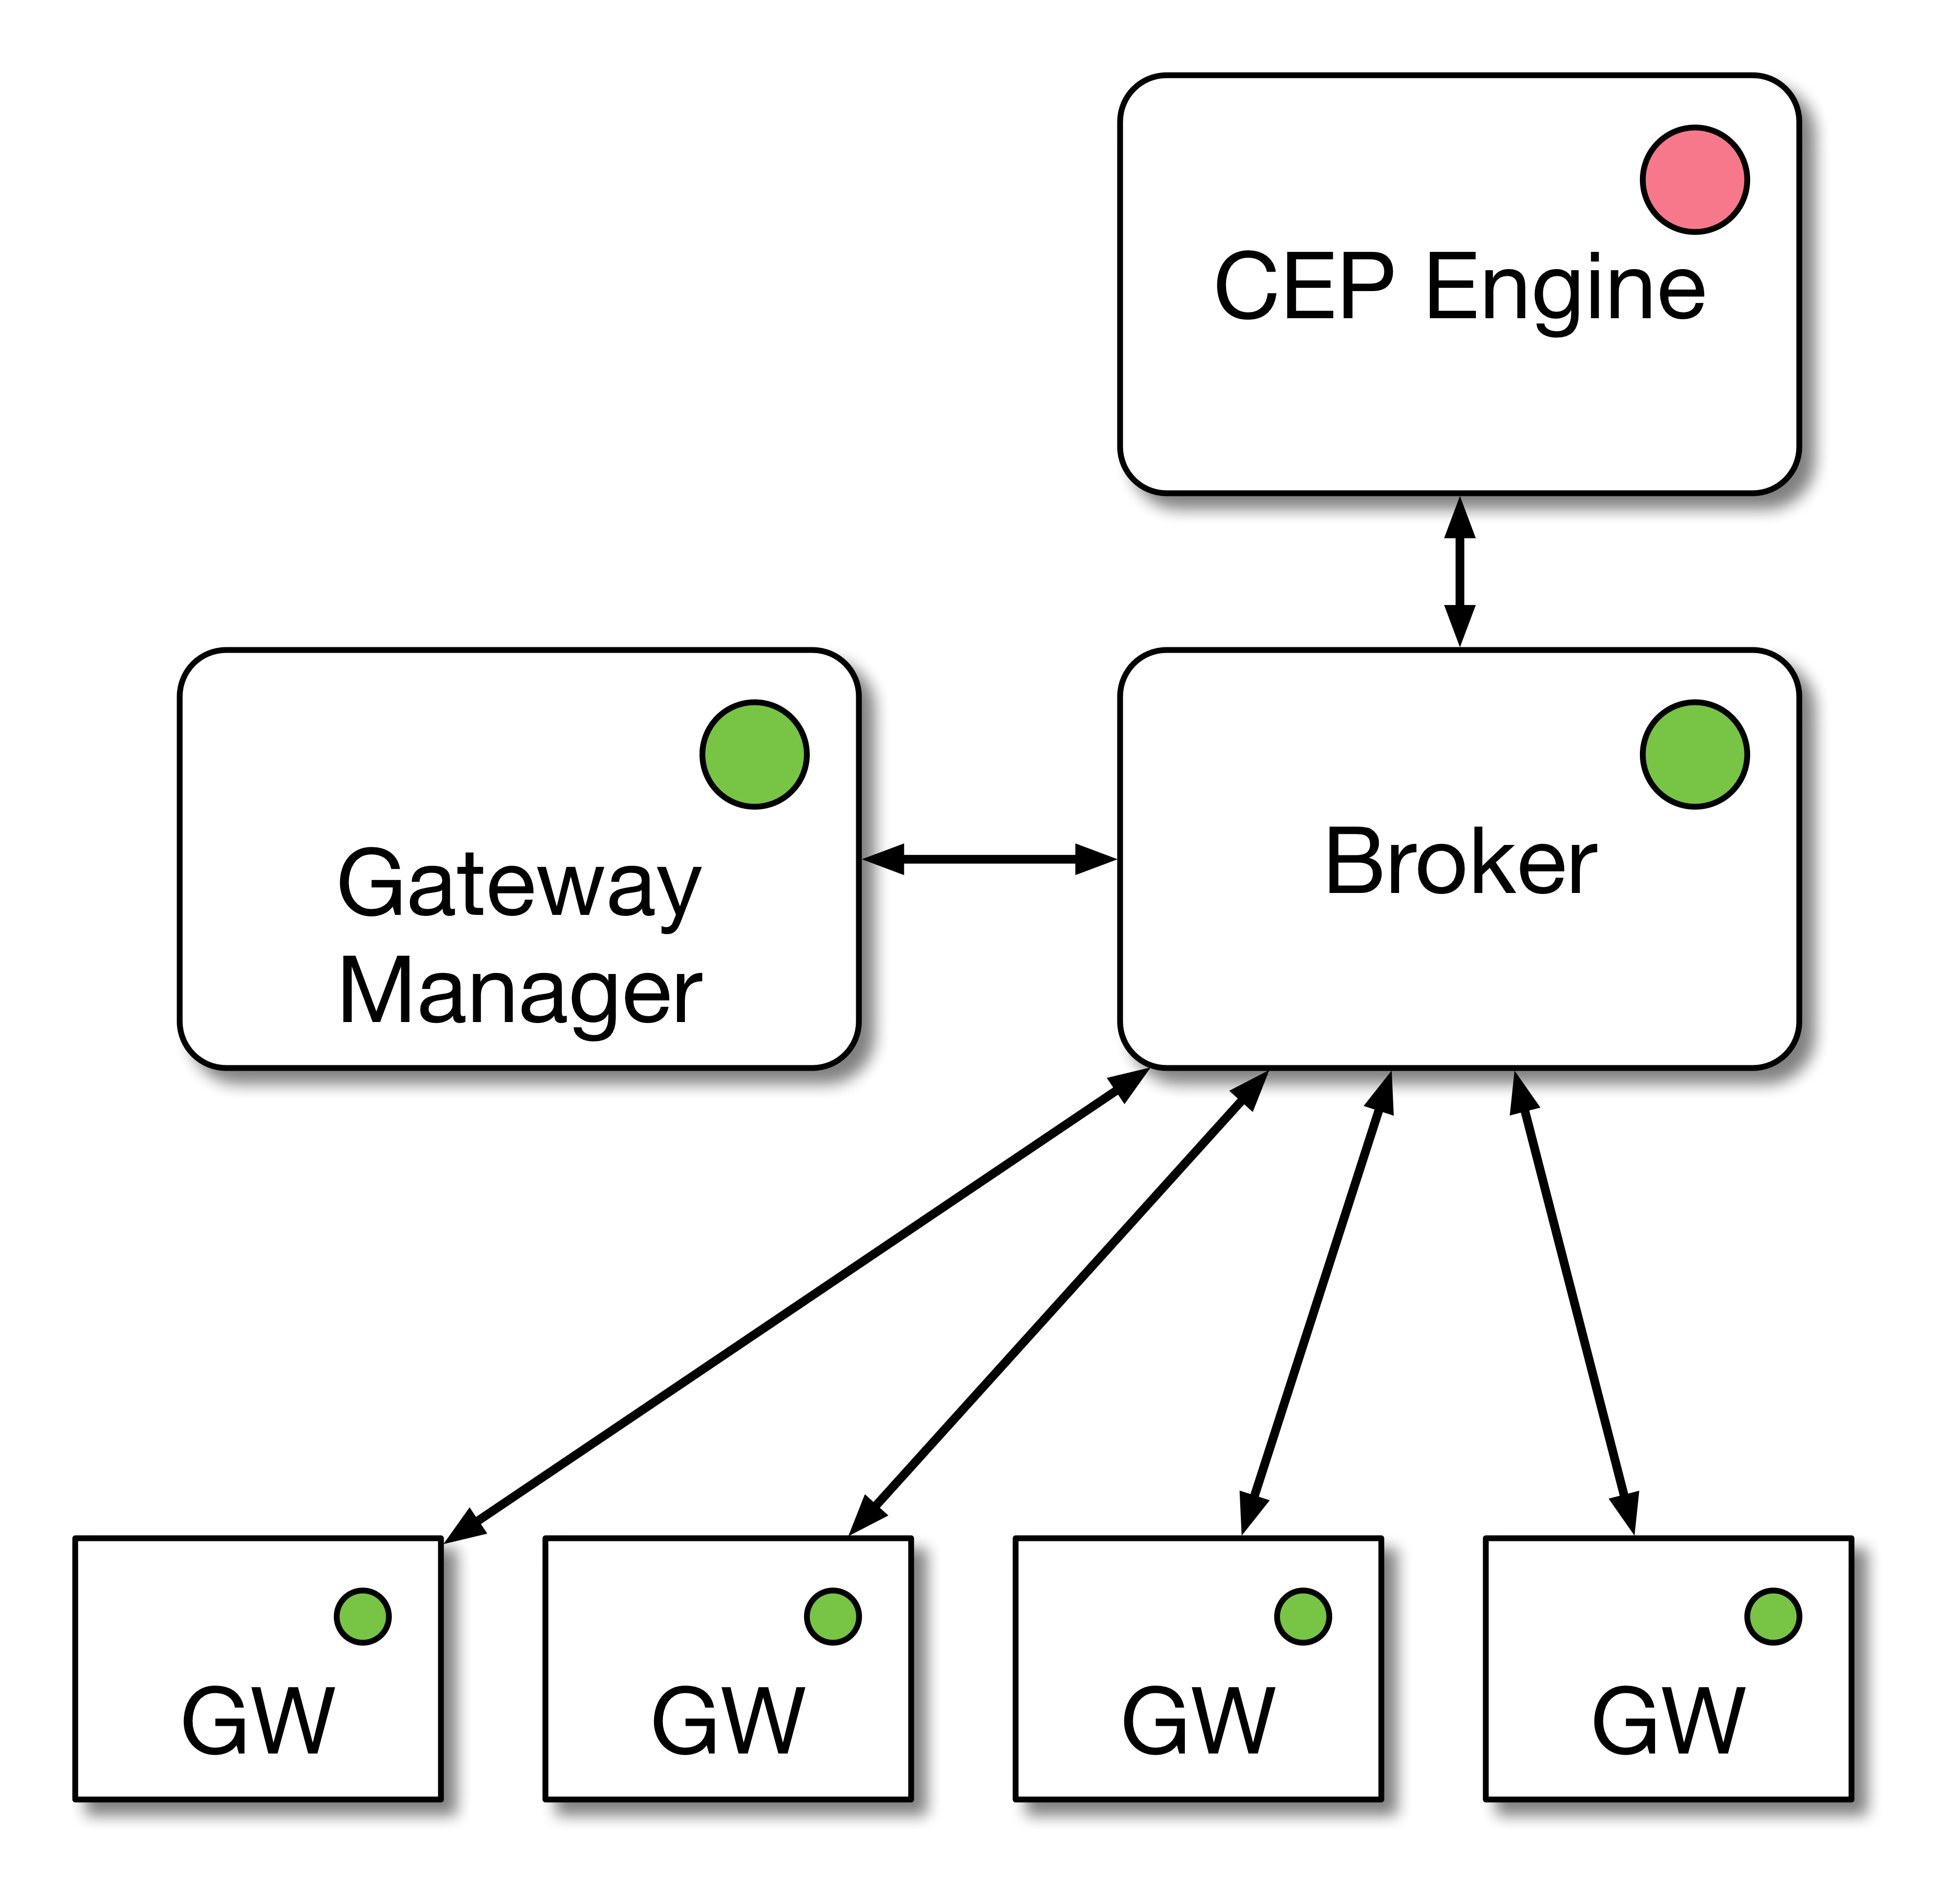
\includegraphics[width=0.4\textwidth]{figures/fs2.png}
		\caption{Functioning scenario 2.}
		\label{fig:sc2}
	\end{figure}
	
	In this second scenario, shown in Figure \ref{fig:sc2}, the CEP module fails and thus, the event processing is halted, either because the server where the program was running was down, or because of a failure in the connection between this component and the message broker. Either way, in this scenario, the generated events cannot reach the CEP Engine to be processed. Since one of the requirements for this project is granting that the building's basic functionalities, like lighting, still work, the system should be able to detect this failure and gateways should begin to process events. 
	
\end{Paragraph}

\begin{Paragraph}{Scenario 3 - Gateway Manager failure}
	
	\begin{figure}[H]
		\centering
		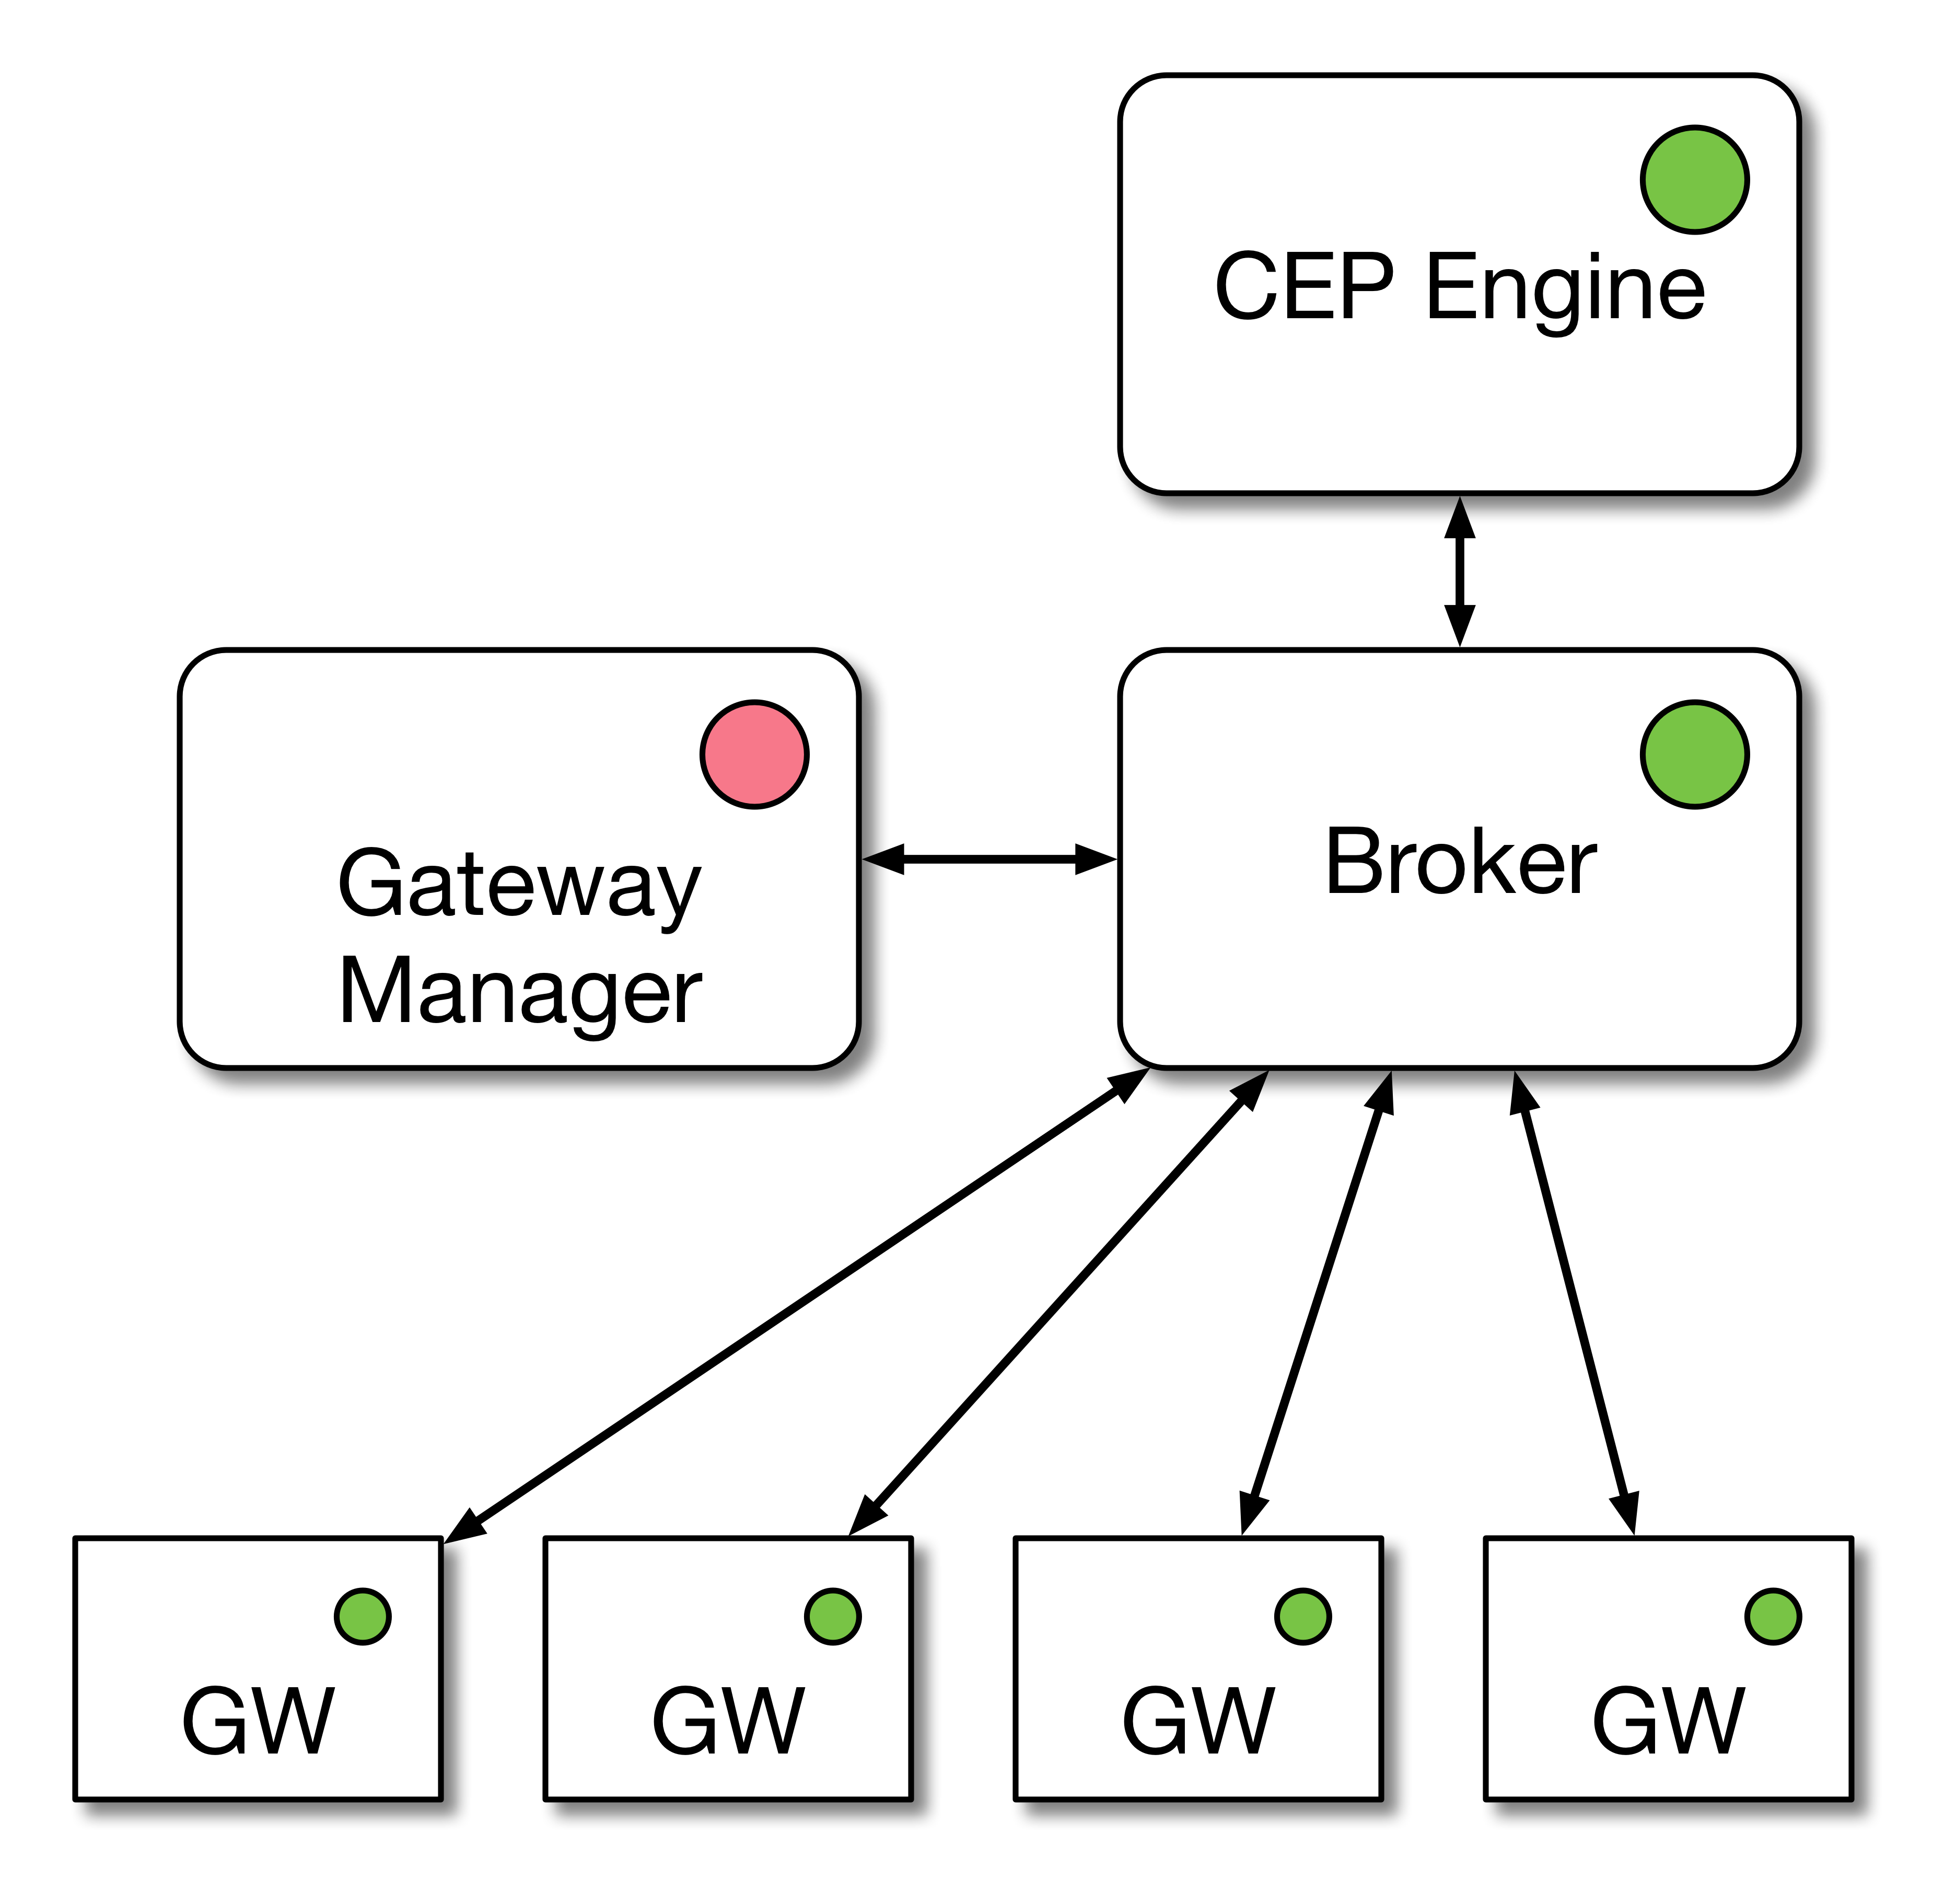
\includegraphics[width=0.4\textwidth]{figures/fs5.png}
		\caption{Functioning scenario 3.}
		\label{fig:sc3}
	\end{figure}
	
	Scenario 3 represents a failure in the Gateway Manager while all the other components are working correctly. Again, this failure can be due to a program error, a downtime in the server where the program is running, or because of a failure in the connection between this component and the message broker. When one of this situations happens, the system should continue to work correctly, however, since this component is responsible for distribute rules and devices through the accessible gateways, this features will not be available and thus, the automation of some building areas might stop working.
	
	
\end{Paragraph}

\begin{Paragraph}{Scenario 4 - Gateway Manager and \ac{cep} Engine failure}
	
	\begin{figure}[H]
		\centering
		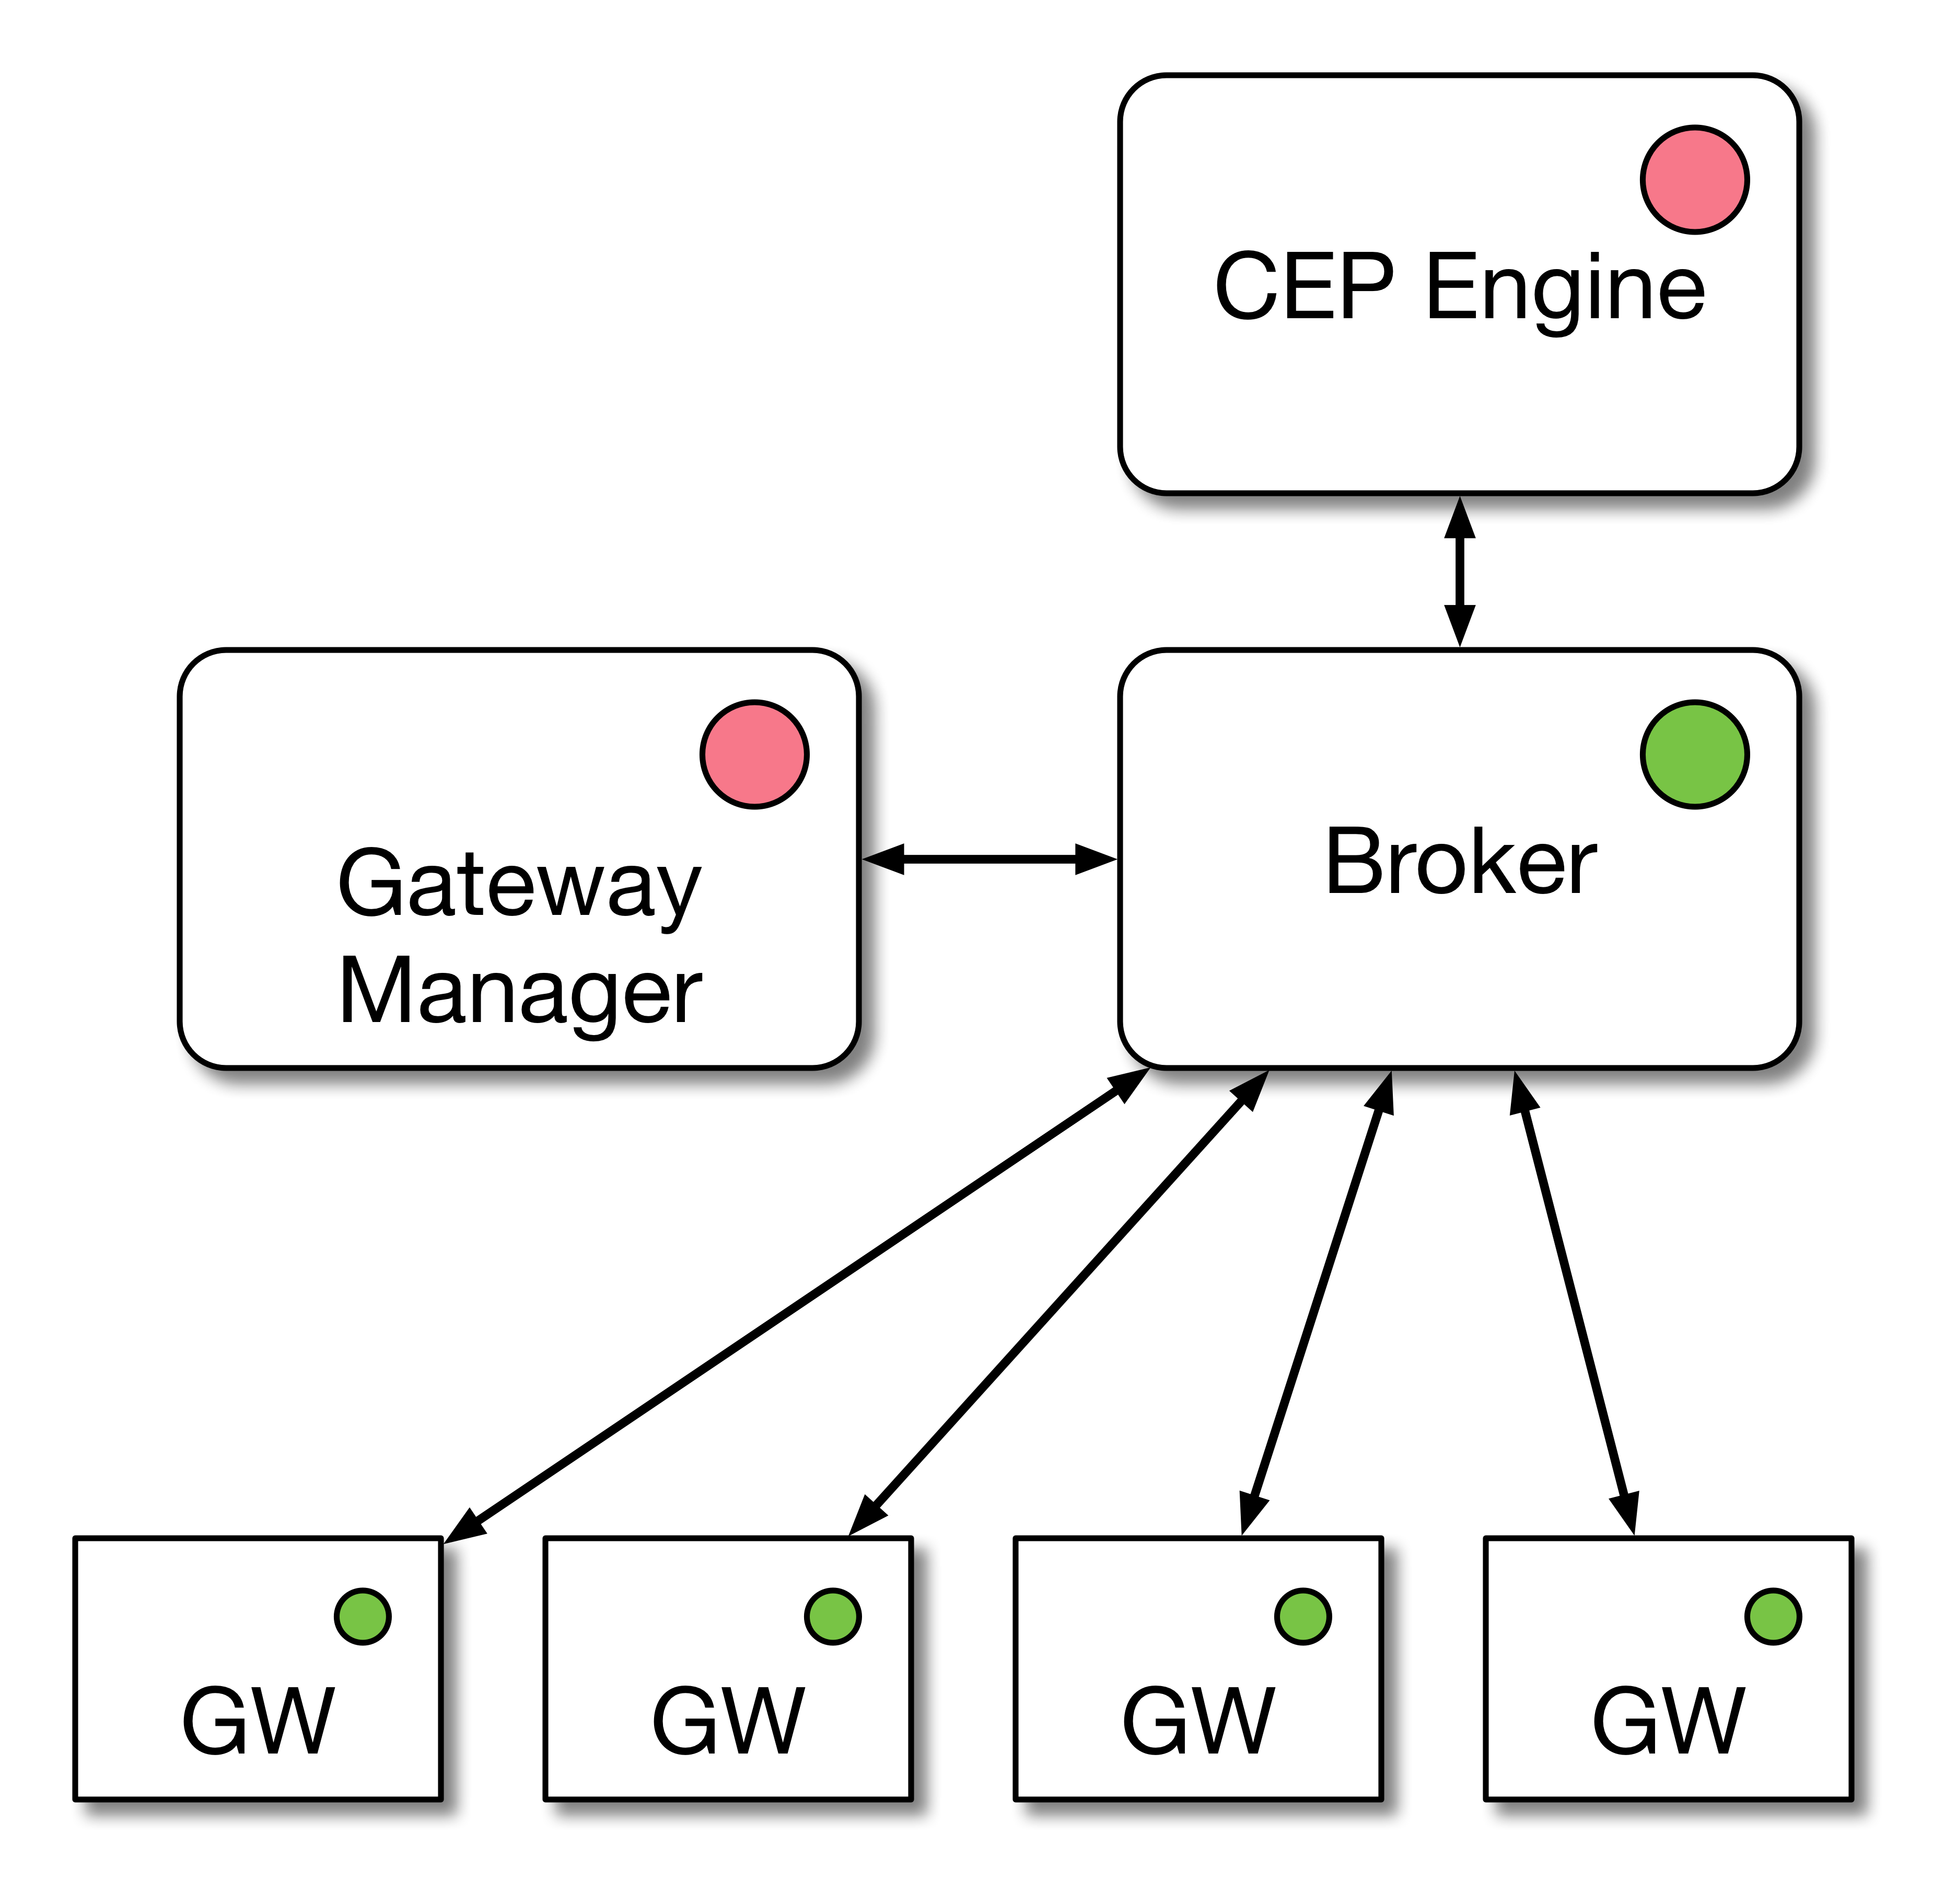
\includegraphics[width=0.4\textwidth]{figures/fs4.png}
		\caption{Functioning scenario 4.}
		\label{fig:sc4}
	\end{figure}
	
	This scenario corresponds to both the Gateway Manager and the \ac{cep} Engine being unavailable. This scenario is a combination of the failures shown in scenario 2 and 3, as both the CEP Engine and the Gateway Manager are no longer disposable. Again, this can happen if the two components fail internally at the same time, or the communication between them and the message broker is down. Based on what each component is responsible for, this scenario would made unavailable the processing of events in the CEP Engine and the rules and devices distribution to gateways performed by the Gateway Manager. In this scenario the system should continue the processing of events in the gateways, and make use, if necessary from the message broker.
	
\end{Paragraph}


\begin{Paragraph}{Scenario 5 - \ac{mqtt} Broker failure}
	
	\begin{figure}[H]
		\centering
		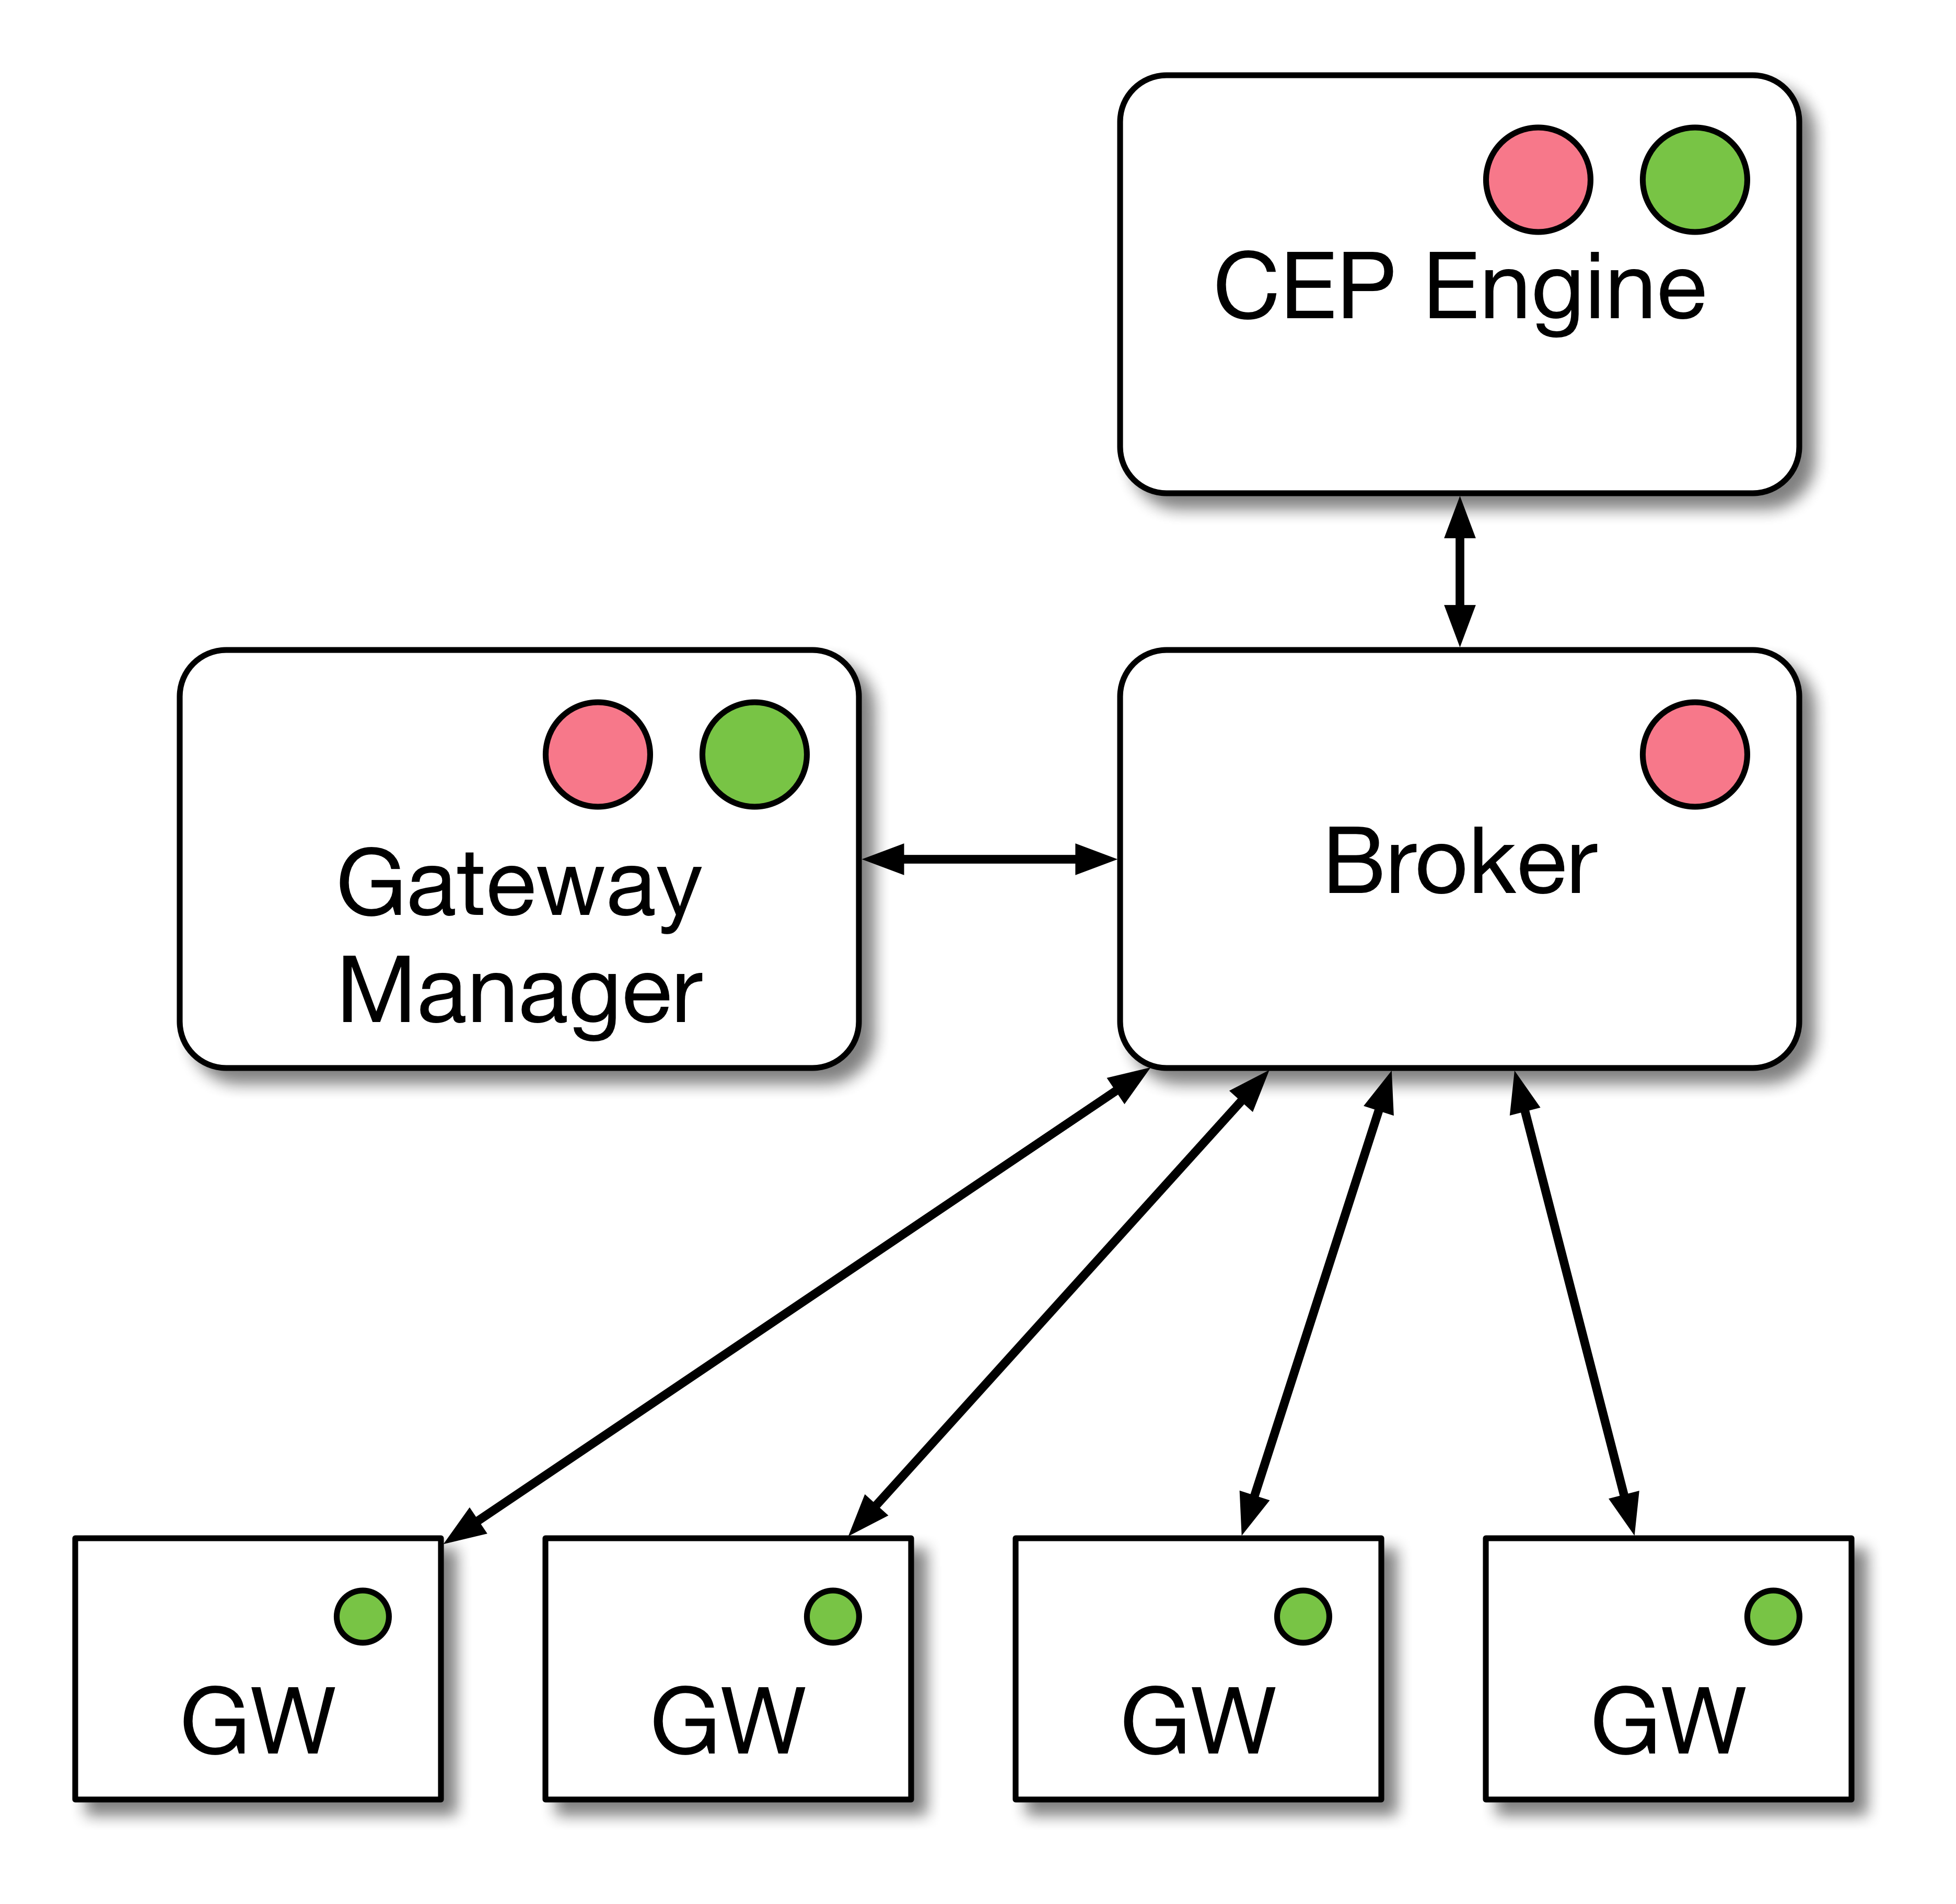
\includegraphics[width=0.4\textwidth]{figures/fs3.png}
		\caption{Functioning scenario 5.}
		\label{fig:sc5}
	\end{figure}
	
	The third scenario, shown in Figure \ref{fig:sc5}, when the broker is down, the communication between gateways and the CEP Engine is cut off, so even if the CEP Engine is still running, it wont be able to process any events generated by the sensors.
	In this scenario, the most severe one, gateways need to be responsible of processing events and apply the rules for the minimum functionality that was described before.
	
\end{Paragraph}


In every scenario stated before there is a need for failure recovery of the gateways too. For instance, if a gateway gets disconnected, the other gateways should be able to take over the sensors and actuators previously owned by the failing gateway and act as gateway for them.







